\section{Тест производительности}
Тест производительности представляет собой сравнение работы многопоточной сортировки слиянием в 1, 2, 3, 4 потока с обычной последовательной сортировкой слиянием, std::sort, sort (bash), линейной сортировкой подсчетом.

Я написала линейную сортировку подсчетом. Так как она не поддерживает отрицательные числа (моя реализация), то тесты были заменены. Отрицательных чисел нет, но размерность тестов сохранилась.
\begin{lstlisting}[language=C]
void CountingSort(std::vector<int64_t>& array, int64_t n) {
    std::vector<int64_t>::iterator iter = std::max_element(array.begin(), array.end());
    int64_t index = std::distance(array.begin(), iter);
    int64_t k = array[index];
    std::vector<int64_t> second(n);
    std::vector<int64_t> c(k + 1, 0);
 
    for (int64_t i = 0; i < n; ++i) {
        ++c[array[i]];
    }
   
    for (int64_t i = 1; i < k + 1; ++i) {
       c[i] += c[i - 1];
    }
  
    for (int64_t i = n; i > 0; --i) {
        second[c[array[i - 1]] - 1] = array[i - 1];
        --c[array[i - 1]];
    }
    for(size_t i = 0; i < n; ++i) {
        array[i] = second[i];
    }
}
\end{lstlisting}

\\Тесты:
\\randtest1kk - 1 миллион строк с рандомными числами;
\\uptest1kk - 1 миллион строк чисел, отсортированных по возрастанию;
\\downtest1kk - 1 миллион строк чисел, отсортированных по убыванию;

\\randtest10kk - 10 миллионов строк с рандомными числами;
\\uptest10kk - 10 миллионов строк чисел, отсортированных по возрастанию;
\\downtest10kk - 10 миллионов строк чисел, отсортированных по убыванию;

\\randtest100kk - 100 миллионов строк с рандомными числами;
\\uptest100kk - 100 миллионов строк чисел, отсортированных по возрастанию;
\\downtest100kk - 100 миллионов строк чисел, отсортированных по убыванию;

\begin{tabular}{ l l l l }
Тесты & randtest1kk & uptest1kk & downtest1kk \\
\\
Parallel Merge Sort 1 thread & 0.169 seconds & 0.086 seconds & 0.09 seconds \\
user & 0m1.790s & 0m1.551s & 0m1.563s & \\
\\
Parallel Merge Sort 2 thread & 0.132 seconds & 0.076 seconds & 0.077 seconds \\
user & 0m1.877s & 0m1.623s & 0m1.733s & \\
\\
Parallel Merge Sort 3 thread & 0.125 seconds & 0.077 seconds & 0.08 seconds \\
user & 0m1.867s & 0m1.668s & 0m1.658s &\\
\\
Parallel Merge Sort 4 thread & 0.132 seconds & 0.084 seconds & 0.085 seconds \\
user & 0m1.905s & 0m1.652s & 0m1.673s \\
\\
Sequal Merge Sort & 0.311 seconds & 0.16 seconds & 0.166 seconds \\
user & 0m1.520s & 0m1.305s & 0m1.335s \\
\\
std::sort & 0.064 seconds & 0.001 seconds & 0.002 seconds \\
user & 0m1.476s & 0m1.370s & 0m1.410s \\
\\
Linear Counting Sort & 100.549 seconds & 103.292 seconds & 111.943 seconds \\
user & 1m20.188s & 1m20.185s & 1m23.227s \\
\\
sort from bash & user 0m1.088s & user 0m1.139s & user 0m2.395s \\
\end{tabular}

\begin{tabular}{ l l l l }
Тесты & randtest10kk & uptest10kk & downtest10kk \\
\\
Parallel Merge Sort 1 thread & 1.933 seconds & 0.996 seconds & 1.041 seconds \\
user & 0m17.965s& 0m15.565s & 0m16.097s & \\
\\
Parallel Merge Sort 2 thread & 1.712 seconds & 0.873 seconds & 0.891 seconds \\
user & 0m19.650s & 0m17.251s & 0m17.403s & \\
\\
Parallel Merge Sort 3 thread & 1.421 seconds & 0.947 seconds & 0.948 seconds \\
user & 0m19.757s & 0m16.966s & 0m17.042s \\
\\
Parallel Merge Sort 4 thread & 1.761 seconds & 0.956 seconds & 1 seconds \\
user & 0m20.170s & 0m17.103s & 0m17.409s \\
\\
Sequal Merge Sort & 3.64 seconds & 1.893 seconds & 1.914 seconds \\
user & 0m16.060s & 0m14.040s & 0m14.080s \\
\\
std::sort & 0.753 seconds & 0.013 seconds & 0.027 seconds \\
user & 0m15.628s & 0m13.713s & 0m13.692s \\
\\
Linear Counting Sort & 189.074 seconds & 146.789 seconds & 132.752 seconds \\
user & 1m55.846s & 1m47.014s & 1m43.623s \\
\\
sort from bash & 0m39.020s &  0m11.415s & 0m12.357s \\
\end{tabular}


\begin{tabular}{ l l l l }
Тесты & randtest100kk & uptest100kk & downtest100kk \\
\\
Parallel Merge Sort 1 thread & 27.144 seconds & 15.489 seconds &  15.404 seconds
user & 2m3.552s & 1m39.435s &  & 1m46.718\\
\\
Parallel Merge Sort 2 thread & 28.346 seconds & 17.309 seconds & 20.238 seconds 
user & 3m51.390s & 3m12.896s & 3m1.880s & \\
\\
Parallel Merge Sort 3 thread & 15.525 seconds & 15.189 seconds &  11.025 seconds
user & 2m6.646s & 1m47.141s & 1m49.376s \\
\\
Parallel Merge Sort 4 thread & 15.33 seconds & 12.502 seconds & 14.46 seconds \\
user & 2m12.633s & 1m57.242s & 1m58.133s \\
\\
Sequal Merge Sort & 45.513 seconds & 34.497 seconds & 24.704 seconds \\
user & 2m59.318s & 2m42.997s & 2m29.869s \\
\\
std::sort & 24.391 seconds & 0.234 seconds & 1.674 seconds \\
user & 3m9.602s & 2m34.925s & 2m29.551s \\
\\
Linear Counting Sort & 1647.64 seconds & 2294.97 seconds & 150.576 seconds \\
user & 7m54.768s & 3m30.745s & 3m38.582s \\
\\
sort from bash & 12m21.939s & 3m24.166s & 3m43.246s \\
\end{tabular}
\\
Самой быстрой сортировкой оказалась std::sort из библиотеки STL. Стандартом не оговаривается, какой именно алгоритм должен быть реализован у std::sort, но сложность обязательно должна быть O(nlogn). Поэтому обычная быстрая сортировка не может быть использована, а Introsort или интроспективная сортировка — использует быструю сортировку и переключается на пирамидальную сортировку, когда глубина рекурсии превысит некоторый заранее установленный уровень (например, логарифм от числа сортируемых элементов). Этот подход сочетает в себе достоинства обоих методов с худшим случаем O(nlogn) и быстродействием, сравнимым с быстрой сортировкой. Могу предположить, что в сортировке предусмотрены критические случаи, для которых придумали нужные и важные оптимизации, что и позволяет этому алгоритму обгонять мою реализацию многопоточного алгоритма слияния. По моему мнению, второе место занимает двухпоточная сортировка слиянием, она показывает довольно стабильные результаты на любых данных, только алгоритм слияния в три потока показывает лучшее время на рандомных тестах, но на отсортированных данных двухпоточная сортировка выигрывает на некоторое количество секунд.

Для сравнения производительности и времени работы моей многопоточной сортировки слиянием я использовала команду sort в bash. Ключ -n нужен для сортировки строк по числовому значению, ключ -o - выводить результат в файл. Она дала средние показатели на тестах в 1 миллион и 10 миллионов данных. Но ужасно себя повела при 100 миллионах рандомных данных, она работала дольше всех, время работы команды sort превышает работу других сортировок почти в 4 раза. К сожалению, я не смогла найти никакой информации об оценке работы алгоритма(ов), который(ые) реализован(ы) внутри.

Хуже всех работает сортировка подсчетом, ее сложность O(k + n), где n - количество элементов, k - наибольший элемент последовательности, который, по сути, отвечает за размерность алфавита. k мог принять наибольшее число в тестах, например, 9 223 372 036 854 775 807 (верхняя граница типа int64\_t), сложив это число с n = 10 000 000, то мы получим число операций явно большее, чем O(nlogn) - сложность при данном n = 10 000 000, за которую работает сортировка слиянием.

Сразу заметна разница между последовательным и параллельным алгоритмом. Многопоточный вариант сортировки слиянием обогнал последовательный метод. Но потраченное именно процессорное время от начала запуска команды time до конца работы у параллельного варианта больше. Дополнительное время могло потратиться из-за издержек на создание и/или порождение новых потоков. Даже, если параллельная программа написана правильно, издержки, создаваемые конкурентными конструкторами, могут перегрузить среду выполнения и производительность программы уменьшится. Поэтому оптимальным решением будет применять параллелизм только в том случае, если размер массива больше порогового (глубина рекурсии), который обычно соответствует количеству ядер, после чего программа возвращается к последовательному алгоритму, что я и применила в решении своей задачи. 
\\
Чтобы оценить производительность, количество затраченной памяти и возможные утечки я использовала утилиту Valgrind.
\begin{alltt}
linuxxxoid@linuxxxoid-MS-7721:~/MAI/DA/CW$ g++ cwda.cpp -std=c++11 -lpthread -o da
linuxxxoid@linuxxxoid-MS-7721:~/MAI/DA/CW$ valgrind ./da test150k
==3271== Memcheck, a memory error detector
==3271== Copyright (C) 2002-2017, and GNU GPL'd, by Julian Seward et al.
==3271== Using Valgrind-3.13.0 and LibVEX; rerun with -h for copyright info
==3271== Command: ./da test150k
==3271==
==3271==
==3271== HEAP SUMMARY:
==3271==     in use at exit: 0 bytes in 0 blocks
==3271==   total heap usage: 143 allocs, 143 frees, 5,500,880 bytes allocated
==3271==
==3271== All heap blocks were freed -- no leaks are possible
==3271==
==3271== For counts of detected and suppressed errors, rerun with: -v
==3271== ERROR SUMMARY: 0 errors from 0 contexts (suppressed: 0 from 0)
\end{alltt}
Так как программа отлажена и работает корректно, то ошибок и утечек памяти не наблюдается.
\\
Для измерения потребления памяти я использовала heap profiler - Massif. Он измеряет сколько памяти в куче задействовала программа.
\begin{alltt}
linuxxxoid@linuxxxoid-MS-7721:~/MAI/DA/CW$ valgrind --tool=massif ./da test150k
==3979== Massif, a heap profiler
==3979== Copyright (C) 2003-2017, and GNU GPL'd, by Nicholas Nethercote
==3979== Using Valgrind-3.13.0 and LibVEX; rerun with -h for copyright info
==3979== Command: ./da test150k
==3979==
==3979==
linuxxxoid@linuxxxoid-MS-7721:~/MAI/DA/CW$ ms_print massif.out.3979 | head --lines=100
--------------------------------------------------------------------------------
Command:            ./da test150k
Massif arguments:   (none)
ms_print arguments: massif.out.3979
--------------------------------------------------------------------------------


    MB
3.223^                                ::::
     |                   :   ::@@@#:@::   ::::@:::::::::::::@@@@@@@@@@@@@@@@@:
     |                   :   : @  # @::   : ::@: :::::::::::@@@              :
     |                   :   : @  # @::   : ::@: :::::::::::@@@              :
     |                   :   : @  # @::   : ::@: :::::::::::@@@              :
     |                   :   : @  # @::   : ::@: :::::::::::@@@              :
     |                   :   : @  # @::   : ::@: :::::::::::@@@              :
     |                   :   : @  # @::   : ::@: :::::::::::@@@              :
     |                   ::::: @  # @::   : ::@: :::::::::::@@@              :
     |                   :  :: @  # @::   : ::@: :::::::::::@@@              :
     |                   :  :: @  # @::   : ::@: :::::::::::@@@              :
     |         :         :  :: @  # @::   : ::@: :::::::::::@@@              :
     |         :         :  :: @  # @::   : ::@: :::::::::::@@@              :
     |         :         :  :: @  # @::   : ::@: :::::::::::@@@              :
     |         :::::::::::  :: @  # @::   : ::@: :::::::::::@@@              :
     |     :   :         :  :: @  # @::   : ::@: :::::::::::@@@              :
     |     :   :         :  :: @  # @::   : ::@: :::::::::::@@@              :
     |     :::::         :  :: @  # @::   : ::@: :::::::::::@@@              :
     |  ::::   :         :  :: @  # @::   : ::@: :::::::::::@@@              :
     | ::  :   :         :  :: @  # @::   : ::@: :::::::::::@@@              :
   0 +----------------------------------------------------------------------->Mi
     0                                                                   507.4

Number of snapshots: 78
 Detailed snapshots: [15, 16 (peak), 19, 29, 53, 63, 73]

--------------------------------------------------------------------------------
  n        time(i)         total(B)   useful-heap(B) extra-heap(B)    stacks(B)
--------------------------------------------------------------------------------
  0              0                0                0             0            0
  1      2,295,368           72,712           72,704             8            0
  2      6,888,963          147,024          146,984            40            0
  3     11,323,552          212,560          212,520            40            0
  4     20,163,283          474,712          474,664            48            0
  5     20,190,769          343,632          343,592            40            0
  6     37,870,161          867,928          867,880            48            0
  7     37,924,271          605,776          605,736            40            0
  8     73,268,702        1,654,360        1,654,312            48            0
  9     73,376,060        1,130,064        1,130,024            40            0
 10    144,105,363        3,227,224        3,227,176            48            0
 11    144,319,217        2,178,640        2,178,600            40            0
 12    164,747,084        2,170,440        2,170,408            32            0
 13    171,399,743        3,376,136        3,375,704           432            0
 14    185,081,897        3,376,208        3,375,760           448            0
 15    188,527,245        3,378,344        3,377,768           576            0
\end{alltt}
(a) график, показывающий потребление памяти во время выполнения программы, и (б) подробную информацию об ответственных местах распределения в различных точках программы, включая точку пикового выделения памяти. Cуществует не более одного пикового снимка. Пиковый снимок является подробным снимком и записывает точку, где потребление памяти было наибольшим. Снимок пика представлен на графике полосой, состоящей из символов «\#».
\\
Callgrind - это инструмент профилирования, который записывает историю вызовов между функциями в ходе выполнения программы в виде графа вызовов.
\\
callgrind\_annotate - эта команда считывает данные профиля и печатает отсортированные списки функций, опционально с примечанием источника. Для графической визуализации данных использовала KCachegrind.
\begin{alltt}
linuxxxoid@linuxxxoid-MS-7721:~/MAI/DA/CW$ valgrind —tool=callgrind ./da test150k
==4294== Callgrind, a call-graph generating cache profiler
==4294== Copyright (C) 2002-2017, and GNU GPL'd, by Josef Weidendorfer et al.
==4294== Using Valgrind-3.13.0 and LibVEX; rerun with -h for copyright info
==4294== Command: ./da test150k
==4294== 
==4294== For interactive control, run 'callgrind_control -h'.
==4294== 
==4294== Events : Ir
==4294== Collected : 532099512
==4294== 
==4294== I refs: 532,099,512
linuxxxoid@linuxxxoid-MS-7721:~/MAI/DA/CW$ callgrind_annotate callgrind.out.4294--------------------------------------------------------------------------------
Profile data file 'callgrind.out.4294' (creator: callgrind-3.13.0)
--------------------------------------------------------------------------------
I1 cache: 
D1 cache: 
LL cache: 
Timerange: Basic block 0 - 100119476
Trigger: Program termination
Profiled target: ./da test150k (PID 4294, part 1)
Events recorded: Ir
Events shown: Ir
Event sort order: Ir
Thresholds: 99
Include dirs: 
User annotated: 
Auto-annotation: off

--------------------------------------------------------------------------------
Ir 
--------------------------------------------------------------------------------
532,099,512 PROGRAM TOTALS
linuxxxoid@linuxxxoid-MS-7721:~/MAI/DA/CW$ kcachegrind ./da test150k
\end{alltt}
\begin{figure}[h]
\center{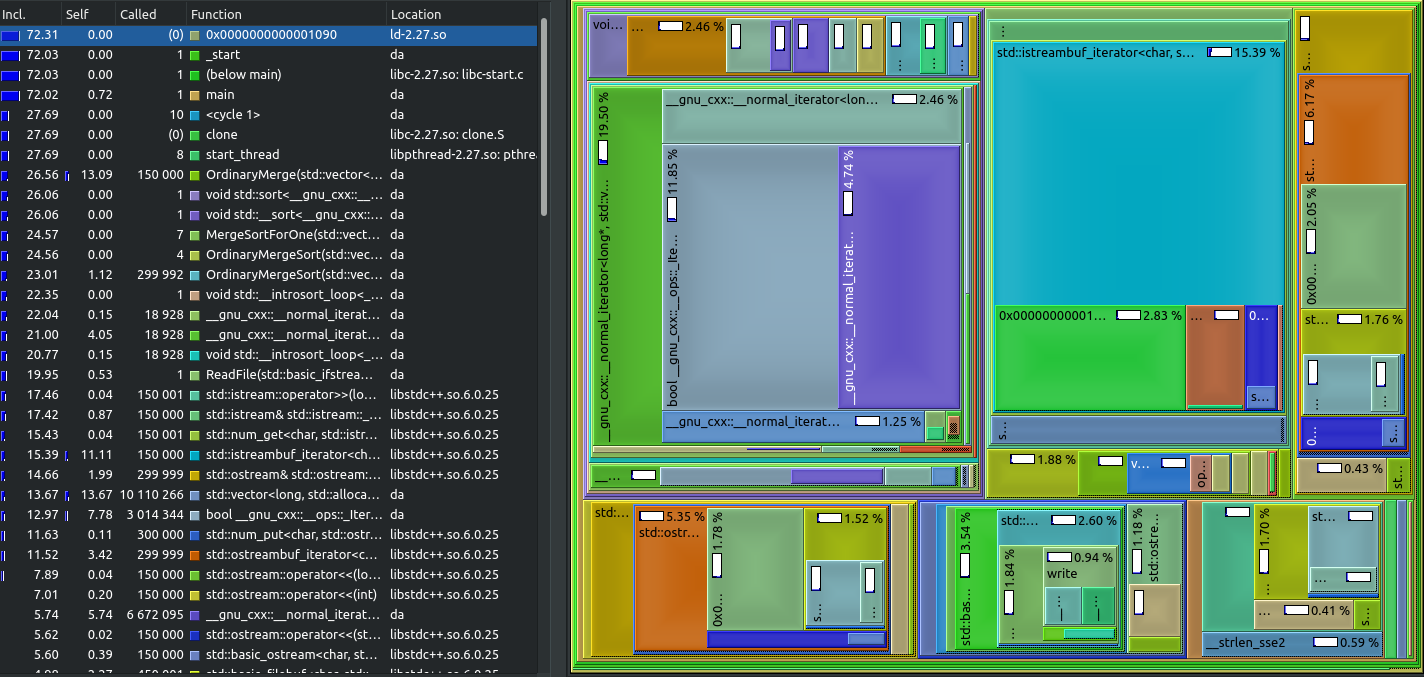
\includegraphics[scale=0.35]{cachgr}}
\end{figure}
\pagebreak